\section{Random.cpp File Reference}
\label{Random_8cpp}\index{Random.cpp@{Random.cpp}}
{\tt \#include \char`\"{}Random.h\char`\"{}}\par


Include dependency graph for Random.cpp:\begin{figure}[H]
\begin{center}
\leavevmode
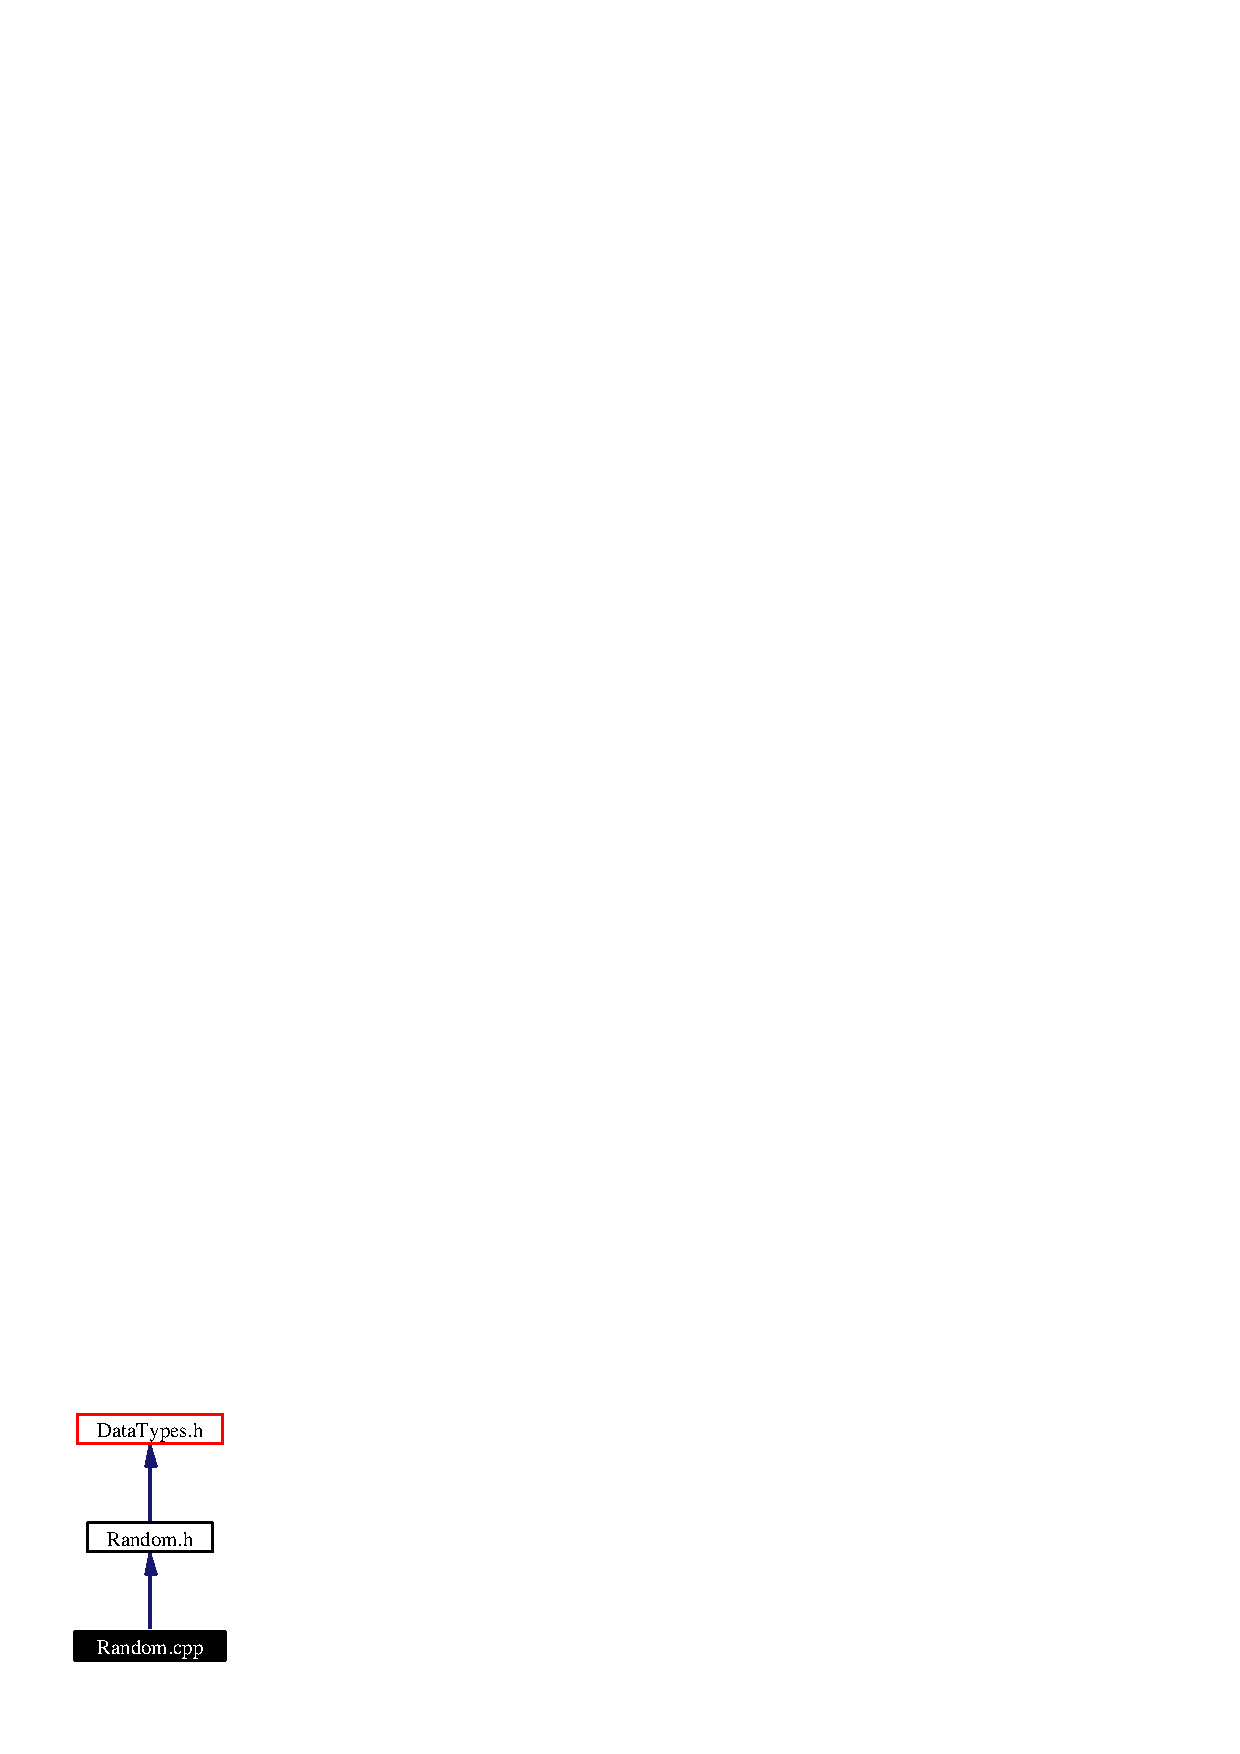
\includegraphics[width=54pt]{Random_8cpp__incl}
\end{center}
\end{figure}
\subsection*{Defines}
\begin{CompactItemize}
\item 
\#define {\bf N}\ 624
\item 
\#define {\bf M}\ 397
\item 
\#define {\bf MATRIX\_\-A}\ 0x9908b0df\-UL
\item 
\#define {\bf UPPER\_\-MASK}\ 0x80000000UL
\item 
\#define {\bf LOWER\_\-MASK}\ 0x7fffffff\-UL
\end{CompactItemize}


\subsection{Define Documentation}
\index{Random.cpp@{Random.cpp}!LOWER_MASK@{LOWER\_\-MASK}}
\index{LOWER_MASK@{LOWER\_\-MASK}!Random.cpp@{Random.cpp}}
\subsubsection{\setlength{\rightskip}{0pt plus 5cm}\#define LOWER\_\-MASK\ 0x7fffffff\-UL}\label{Random_8cpp_a4}




Definition at line 41 of file Random.cpp.

Referenced by dg::Random\-Int().\index{Random.cpp@{Random.cpp}!M@{M}}
\index{M@{M}!Random.cpp@{Random.cpp}}
\subsubsection{\setlength{\rightskip}{0pt plus 5cm}\#define M\ 397}\label{Random_8cpp_a1}




Definition at line 38 of file Random.cpp.

Referenced by dg::Random\-Int().\index{Random.cpp@{Random.cpp}!MATRIX_A@{MATRIX\_\-A}}
\index{MATRIX_A@{MATRIX\_\-A}!Random.cpp@{Random.cpp}}
\subsubsection{\setlength{\rightskip}{0pt plus 5cm}\#define MATRIX\_\-A\ 0x9908b0df\-UL}\label{Random_8cpp_a2}




Definition at line 39 of file Random.cpp.

Referenced by dg::Random\-Int().\index{Random.cpp@{Random.cpp}!N@{N}}
\index{N@{N}!Random.cpp@{Random.cpp}}
\subsubsection{\setlength{\rightskip}{0pt plus 5cm}\#define N\ 624}\label{Random_8cpp_a0}




Definition at line 37 of file Random.cpp.

Referenced by dg::Random\-Int(), and dg::Seed\-Random().\index{Random.cpp@{Random.cpp}!UPPER_MASK@{UPPER\_\-MASK}}
\index{UPPER_MASK@{UPPER\_\-MASK}!Random.cpp@{Random.cpp}}
\subsubsection{\setlength{\rightskip}{0pt plus 5cm}\#define UPPER\_\-MASK\ 0x80000000UL}\label{Random_8cpp_a3}




Definition at line 40 of file Random.cpp.

Referenced by dg::Random\-Int().